\section{Funzionamento di base del sistema DecaWave EVB1000}
\begin{frame}{Introduzione}
  Il sistema di tag ed ancore DecaWave EVB1000 consente di localizzare
  un agente attraverso ricetrasmettitori che implementano la tecnica di trasmissione
  \alert{UWB} (Ultra-wideband).\\
  Alla base del funzionamento del sistema vi è lo scambio di messaggi, tra tag e ancore,
  contententi principalmente informazioni di natura temporale. Tali informazioni consentono
  alle ancore di calcolare il tempo di volo tra esse e il tag e quindi, mediante opportuno
  algoritmo di trialaterazione, di calcolare la posizione del tag.
\end{frame}

\begin{frame}{Two-way Ranging}
  Lo scambio di messaggi avviene secondo il metodo detto \alert{Two-way Ranging}.\\
  Nel dettaglio vengono scambiati, tra tag e ciascuna ancora,
  un messaggio di Poll, uno di Risposta ed uno di Final.\\
  I messaggi di \alert{Poll} e \alert{Final} vengono inviati dal tag
  mentre ogni ancora invia il messaggio di \alert{Risposta}.
  \begin{center}
    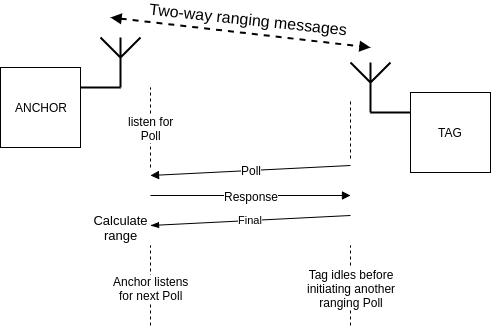
\includegraphics[height=10em]{ranging.png}
  \end{center}
\end{frame}

\begin{frame}{Struttura di un messaggio ed RMARKER}
  La struttura dei messaggi scambiati da tag e ancore è la seguente.
  \begin{center}
    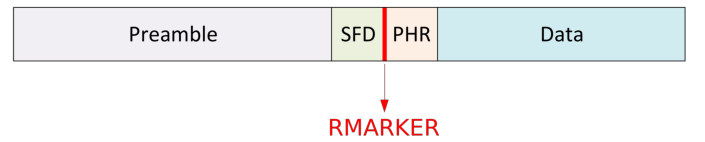
\includegraphics[width=\linewidth]{whole_msg_decawave}
  \end{center}
  Il campo \alert{Data} contiene i dati veri e propri scambiati tra i dispositivi.\\
  Durante la trasmissione di un messaggio l'inizio della parte PHR (PHY header)
  costituisce l'evento da utilizzare per il time-stamping come da standard
  IEEE 802.15.4 UWB PHY. Il tempo, espresso nell'orologio locale del dispositvo, di invio
  del primo simbolo del PHR sarà definito nel seguito \alert{RMARKER}.
\end{frame}

\begin{frame}{Two-way Ranging}
  \begin{columns}[T]
    \begin{column}{0.5\textwidth}
      il \alert{tag} salva RMARKER di
      \begin{itemize}
      \item[-] invio Poll ($Rm_{ps}$)
      \item[-] ricezione Risposta ($Rm_{rr}$)
      \item[-] invio Final ($Rm_{fs}$) (delayed transmission)
      \end{itemize}
    \end{column}
    \begin{column}{0.5\textwidth}
      l'\alert{ancora} salva RMARKER di
      \begin{itemize}
      \item[-] ricezione Poll ($Rm_{pr}$)
      \item[-] spedizione Risposta ($Rm_{rs}$)
      \item[-] ricezione Final ($Rm_{fr}$)
      \end{itemize}
    \end{column}
  \end{columns}
  \begin{center}
    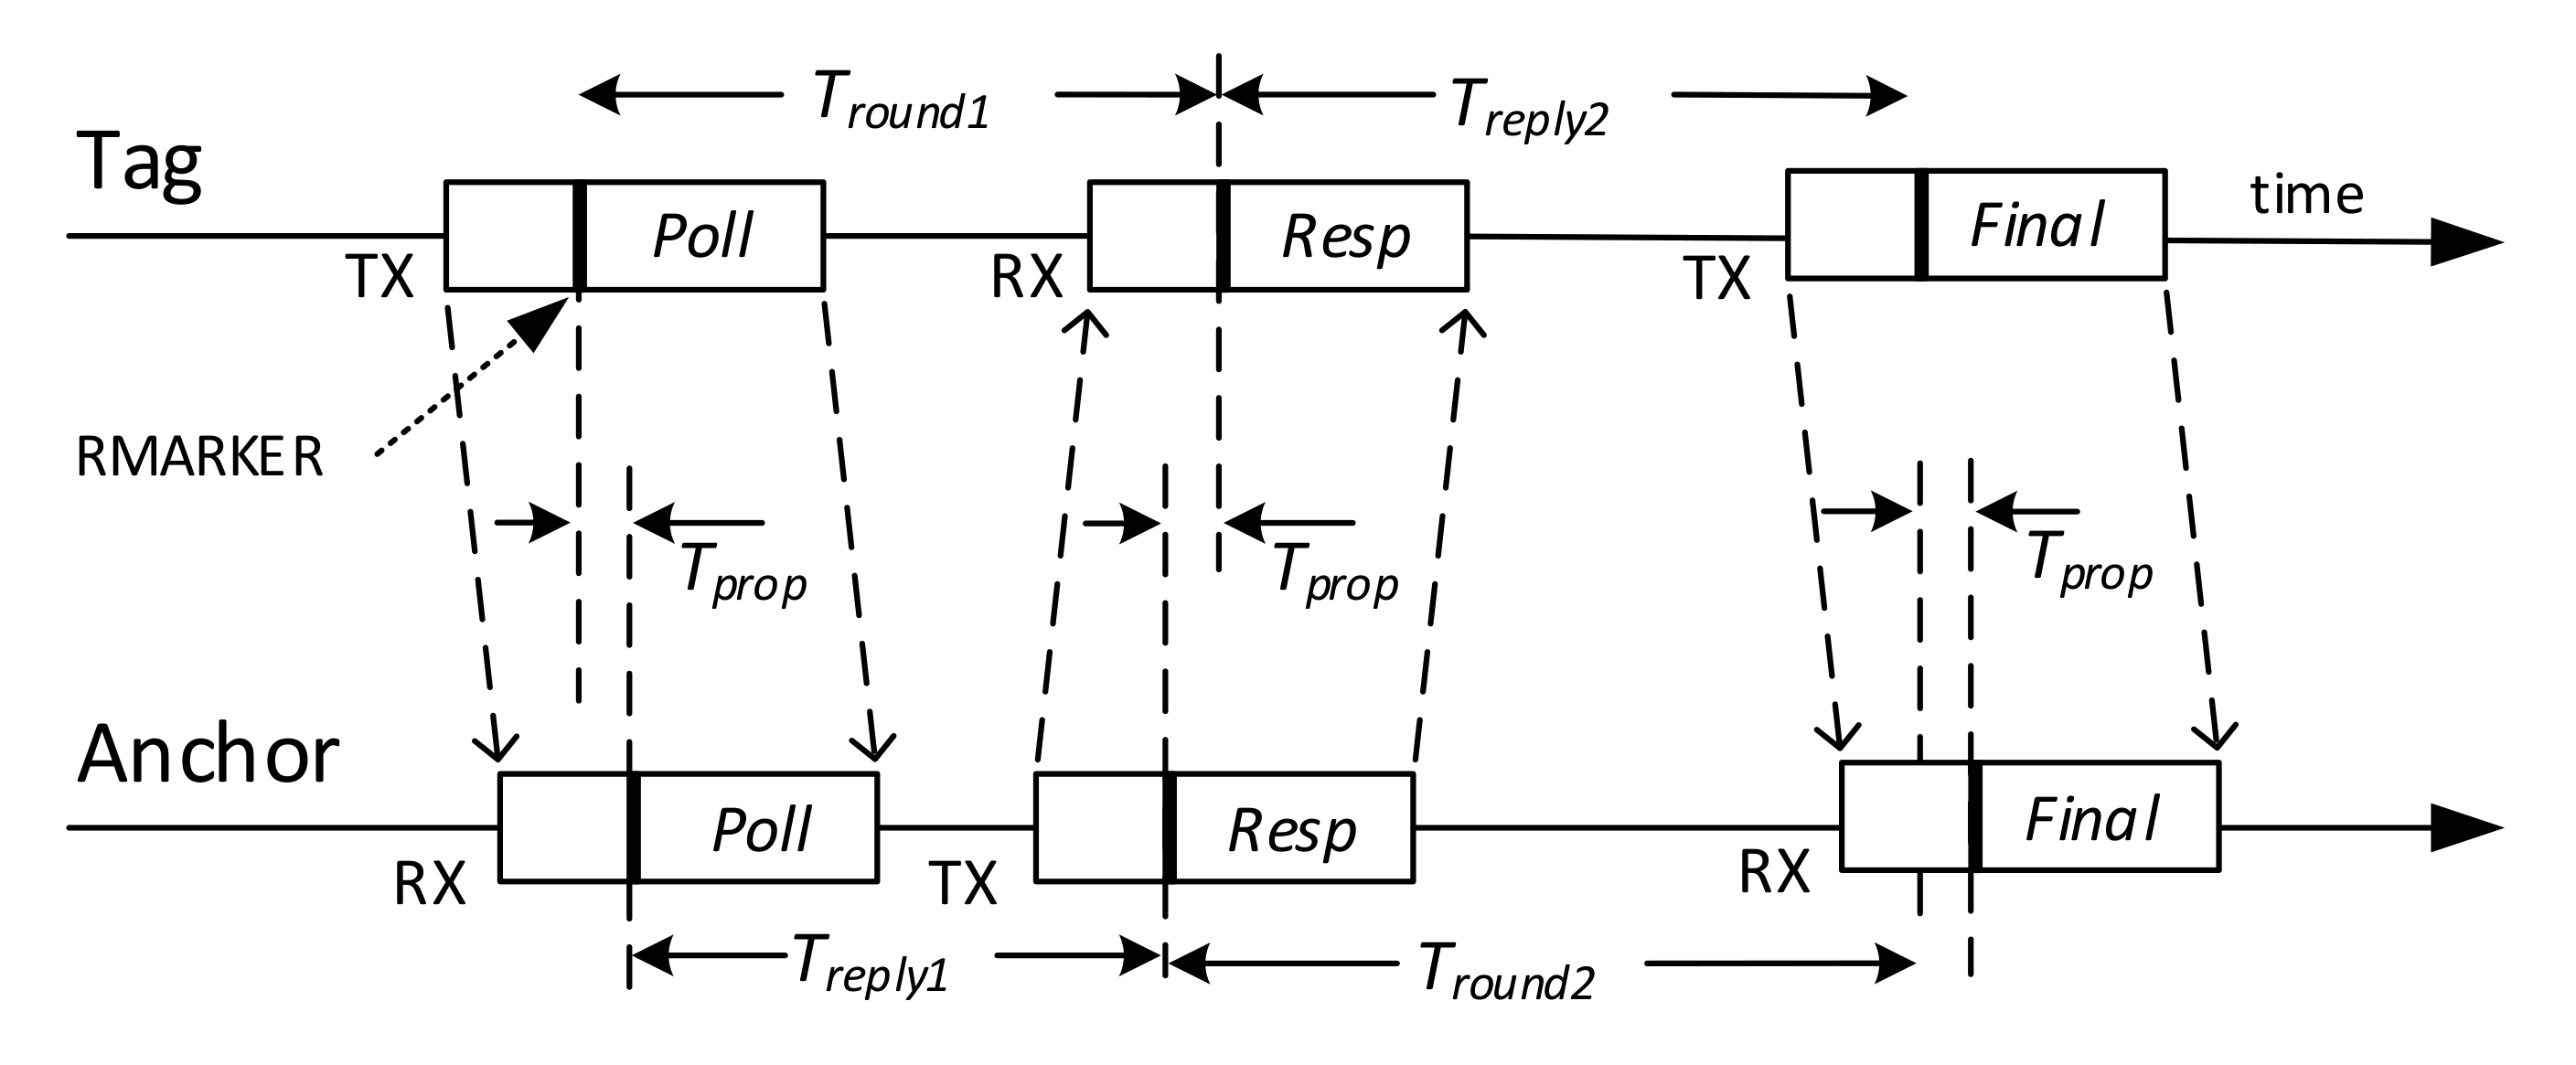
\includegraphics[scale = 0.7]{ranging_with_timings.png}
  \end{center}
  Il tag invia $Rm_{ps}$, $Rm_{rr}$ e $Rm_{fs}$ all'ancora nel Final.
\end{frame}

\begin{frame}{Calcolo del ToF}
  Le seguenti quantità sono \alert{calcolate} dall'\alert{ancora} utilizzando i dati raccolti e
  ricevuti dal tag durante un'istanza di ranging
  \[
  \begin{split}
    T_{round1} = Rm_{rr} - Rm_{ps} \quad \quad T_{round2} = Rm_{fs} - Rm_{rr}\\
    T_{reply1} = Rm_{rs} - Rm_{pr} \quad \quad T_{reply2} = Rm_{fr} - Rm_{rs}
  \end{split}
  \]

  Alla ricezione del Final l'ancora calcola il nuovo Tof ($T_{prop}$) che viene inviato al tag nella Risposta al Poll dell'istanza di ranging \alert{successiva}
  \[
  T_{prop} = \frac{T_{round1} T_{round2} - T_{reply1} T_{reply2}}{T_{round1} + T_{round2} + T_{reply1} + T_{reply2}}
  \]
\end{frame}

\begin{frame}[label={delayed_tx}]{Delayed transmission}
  \begin{alertblock}{Attenzione}
    La necessità di spedire nel messaggio di Final il tempo di spedizione del medesimo richiede
    l'utilizzo della funzione di \emph{delayed transmission} del DW1000.
  \end{alertblock}
  Il tempo di spedizione viene scelto a priori come
  \[
  Rm_{fs} = Rm_{ps} + T_{fd}
  \]
  dove $T_{fd}$ è maggiore del tempo impiegato da \alert{tutte le ancore} per rispondere al tag ed è indicato
  con Final Delay.
  La funzione di \emph{delayed transmission} garantisce che l'RMARKER di spedizione del Final coincida con
  $Rm_{fs}$.
\end{frame}

\begin{frame}{Superframe e frame}
  Durante la trasmissione dei dati i tag e le ancore osservano un protocollo di trasmissione
  \alert{a divisione di tempo} per evitare che un dispositivo possa interferire con la trasmissione
  di un altro.\\
  Nel dettaglio il tempo è diviso in una serie di \alert{superframe} a loro volta divisi in
  frame.\\
  Il firmware originale prevede 10 frame della durata di \SI{10}{\milli\second}, otto dei quali
  sono dedicati ad altrettante istanze di ranging, una per ciascunx tag. I restanti due sono dedicati
  alla ``vecchia'' procedura di ranging tra le ancore. In totale ciascun superframe ha un durata di \SI{100}{\milli\second}.\\
  La configurazione del firmware originale prevede quindi fino a $8$ tag e $3$/$4$ ancore.
\end{frame}

\begin{frame}{Esempio di temporizzazione}
  Un esempio di temporizzazione è mostrato di seguito.
  \centering
  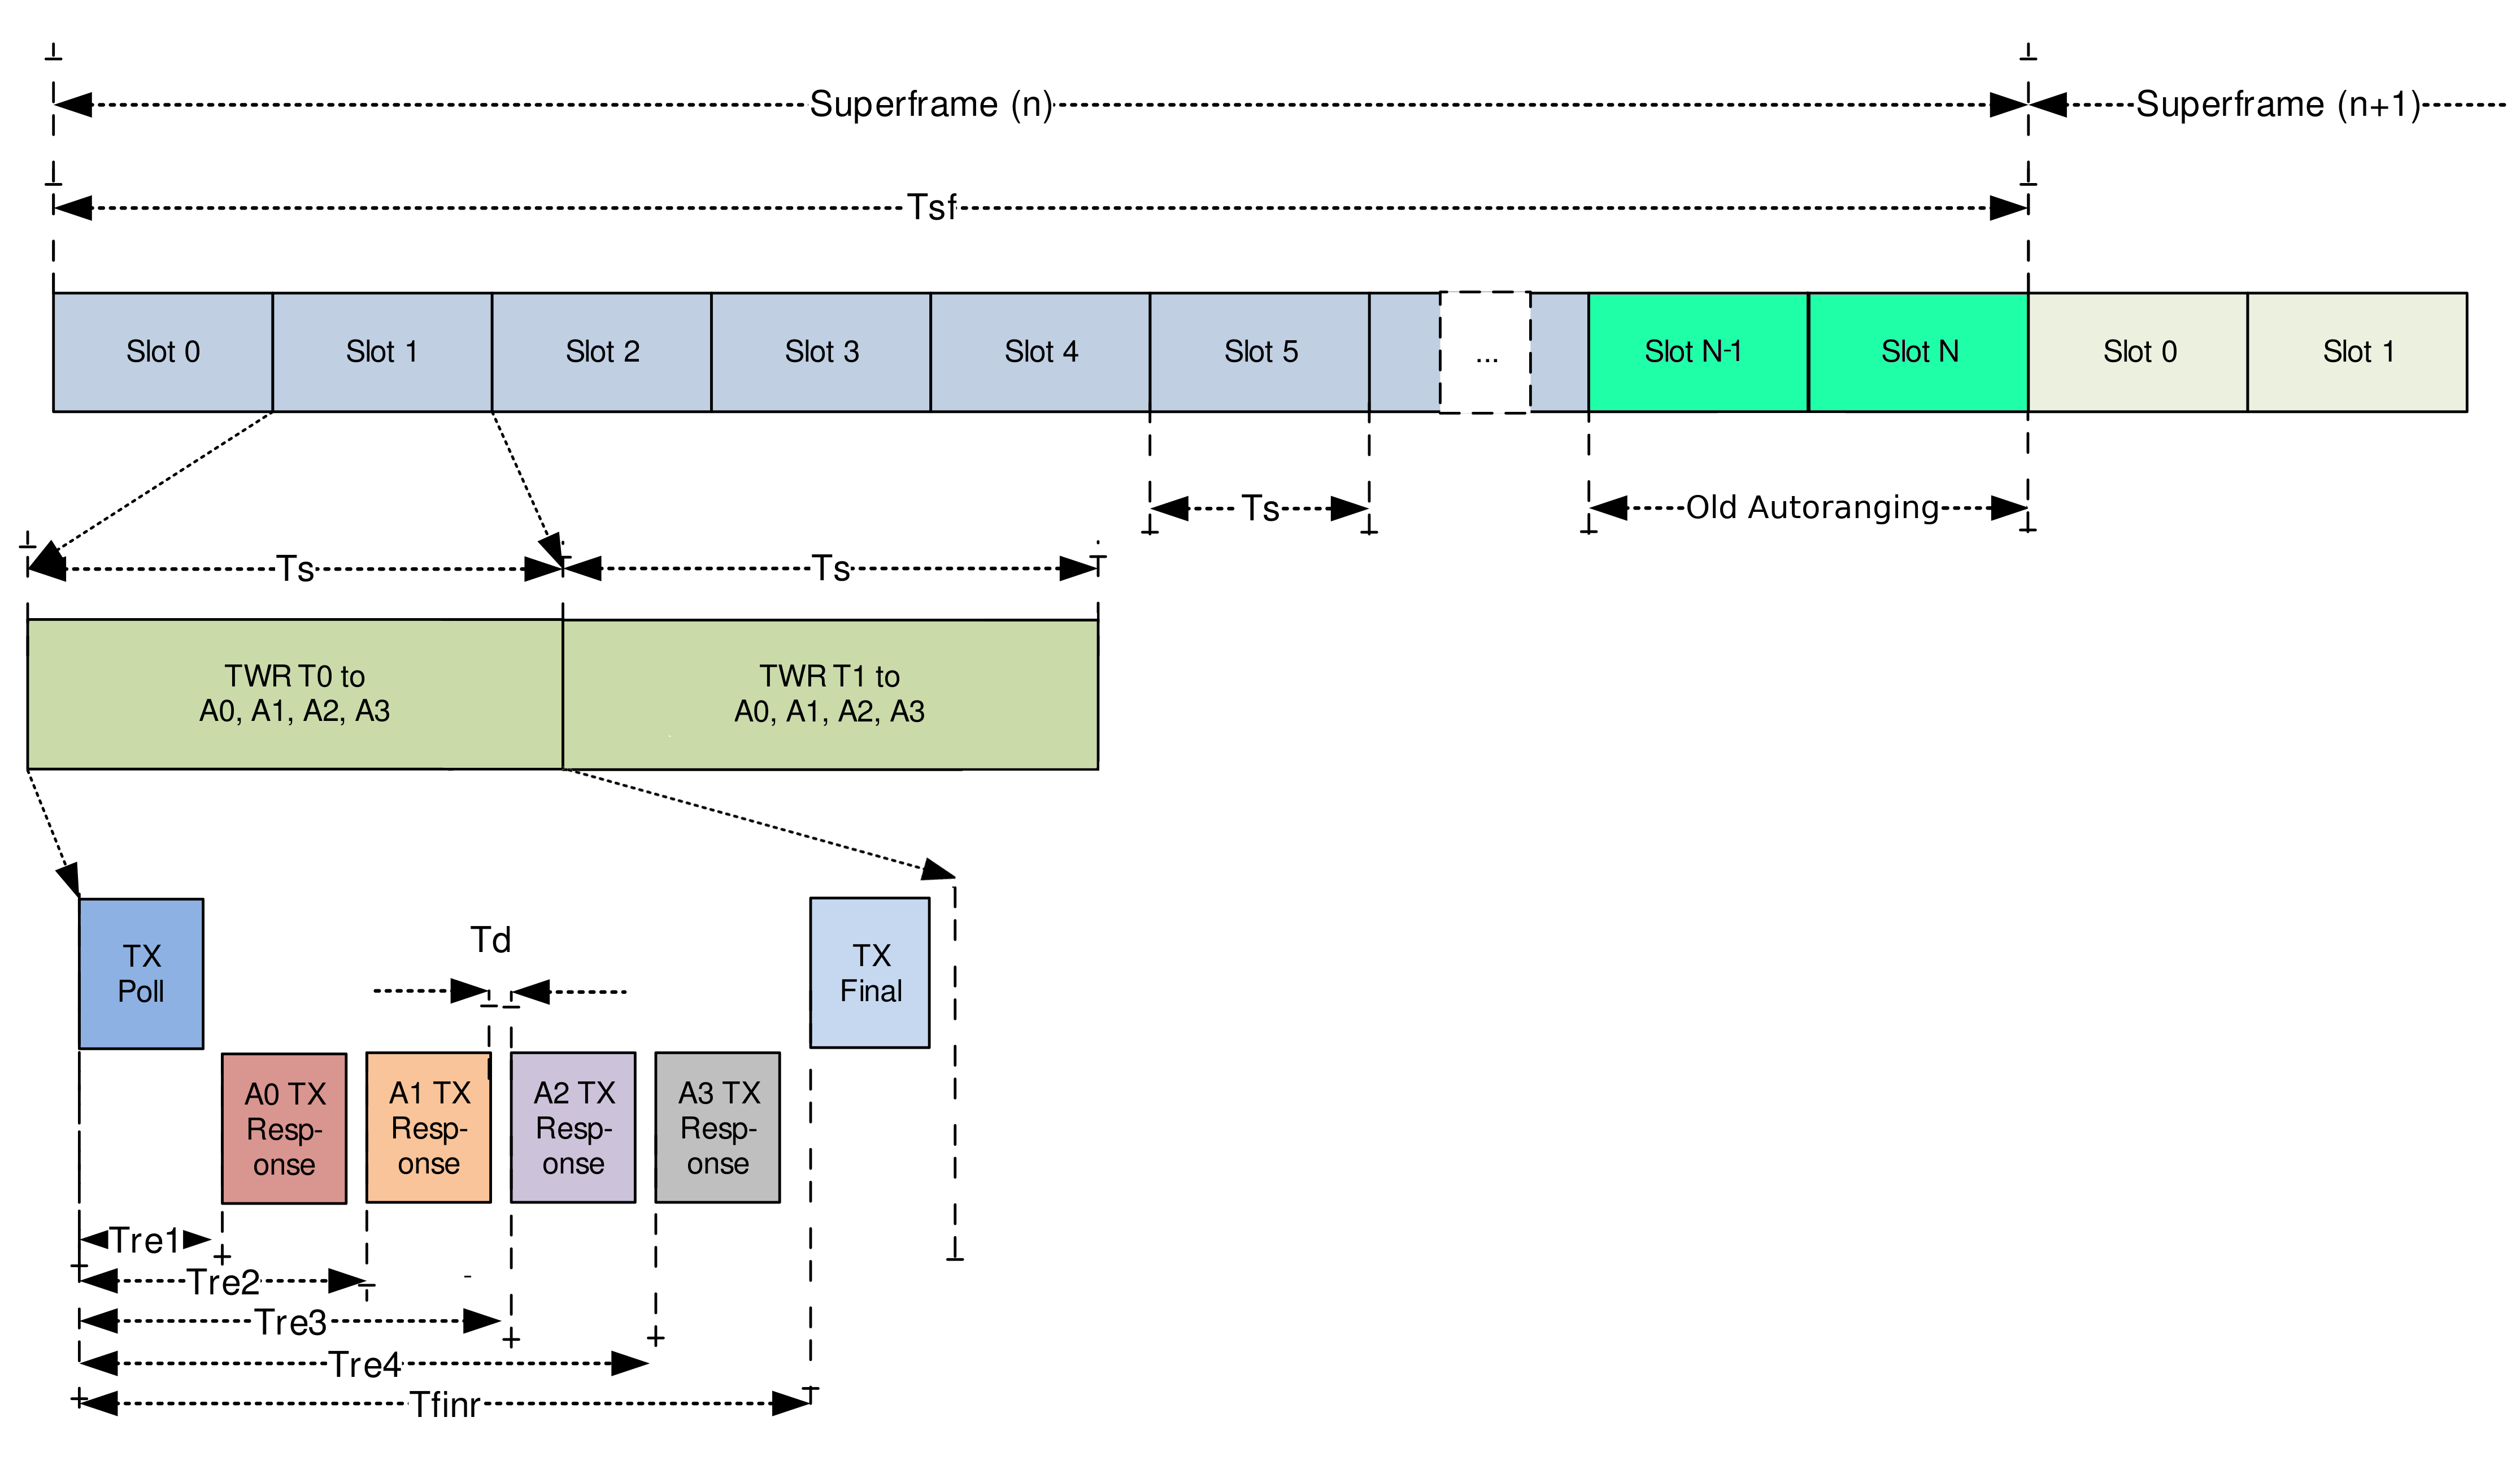
\includegraphics[width=\linewidth]{frame_superframe_a2a.png}
\end{frame}

\begin{frame}[shrink=10, label={anchors_responses_turn}]{Gestione delle risposte delle ancore}
  Come visibile dallo schema riportato nella slide precedente le ancore rispondono una dopo l'altra a partire
  dall'ancora A0.\\
  Per far si che tale ordine sia rispettato ogni ancora, dopo aver ricevuto il messaggio di Poll, sta in ascolto
  delle risposte di tutte le altre ancore. Nel caso ideale in cui tutte le ancore rispondono, l'ancora i-esima
  invia la sua riposta quando la seguente condizione viene verificata
  \[
  N + I = M
  \]
  dove $N$ rappresenta il numero di risposte che l'ancora i-esima si aspetta ancora di ricevere,
  $I$ è l'ID dell'ancora (nel caso di $4$ ancore l'ID è un intero compreso tra $0$ e $3$) ed $M$
  è il numero totale di risposte che l'ancora attende.\\
  Nel caso in cui una delle risposte non arrivi il sistema prevede un meccanismo di timeout che consente
  all'ancora i-esima di inviare comunque la risposta nel momento giusto.
\end{frame}

\begin{frame}{Gestione di più tag}
  Al fine di rendere effettivo il protocollo di trasmissione a divisione di tempi
  l'ancora A0 ricopre un ruolo di arbitraggio. In particolare corregge i tempi di attivazione
  di ogni tag come spiegato di seguito.\\
  Ogni tag invia un messaggio di Poll ogni \alert{activation period} $a_p$
  \[
  a_p = T_{sp} + T_{sr} + T_{sc}
  \]
  \begin{itemize}
  \item[-] $T_{sp}$: periodo ideale di attivazione (detto Sleep Poll) $ = T_{sf}$ : durata del Superframe 
  \item[-] $T_{sr}$: alla prima iterazione vale $\SI{10}{\milli\second}$ successivamente vale  $\SI{0}{\milli\second}$
    (detto Sleep Random)
  \item[-] $T_{sc}$: correzione calcolata dall'\alert{Ancora 0} ed inviata al \alert{tag i-esimo} (detto Sleep Correction)
  \end{itemize}
\end{frame}

\begin{frame}{Calcolo della correzione $T_{sc}$}
  La correzione viene calcolata in base ad un errore calcolato come la differenza tra il tempo atteso
  d'arrivo del Poll e quello effettivo (dal punto di vista dell'ancora 0)
  \[
  e = t_{i}^{a} - t_{rx}
  \]
  La correzione vale
  \[
  \begin{cases}
    T_{sc} = e \quad \quad \quad \quad \text{se } e < -\frac{T_{sf}}{2}\\
    T_{sc} = T_{sf} + e \quad \quad \text{altrimenti}
  \end{cases}
  \]
\end{frame}

\begin{frame}{Calcolo Calcolo del tempo di attivazione $T_{sc} = e$}
  Nel seguente esempio si considera il caso $e < -\frac{T_{sf}}{2}$.\\
  Il tempo di riattivazione del tag $t_{i+1}^{t}$ è:
  \[
  t_{i+1}^{t} = t_{i}^{t} + T_{sf} + T_{sc} = t_i^a - (\cancel{e} + Tof) + T_{sf} + \cancel{e} = t_i^a - Tof + T_{sf} 
  \]
  \begin{center}
    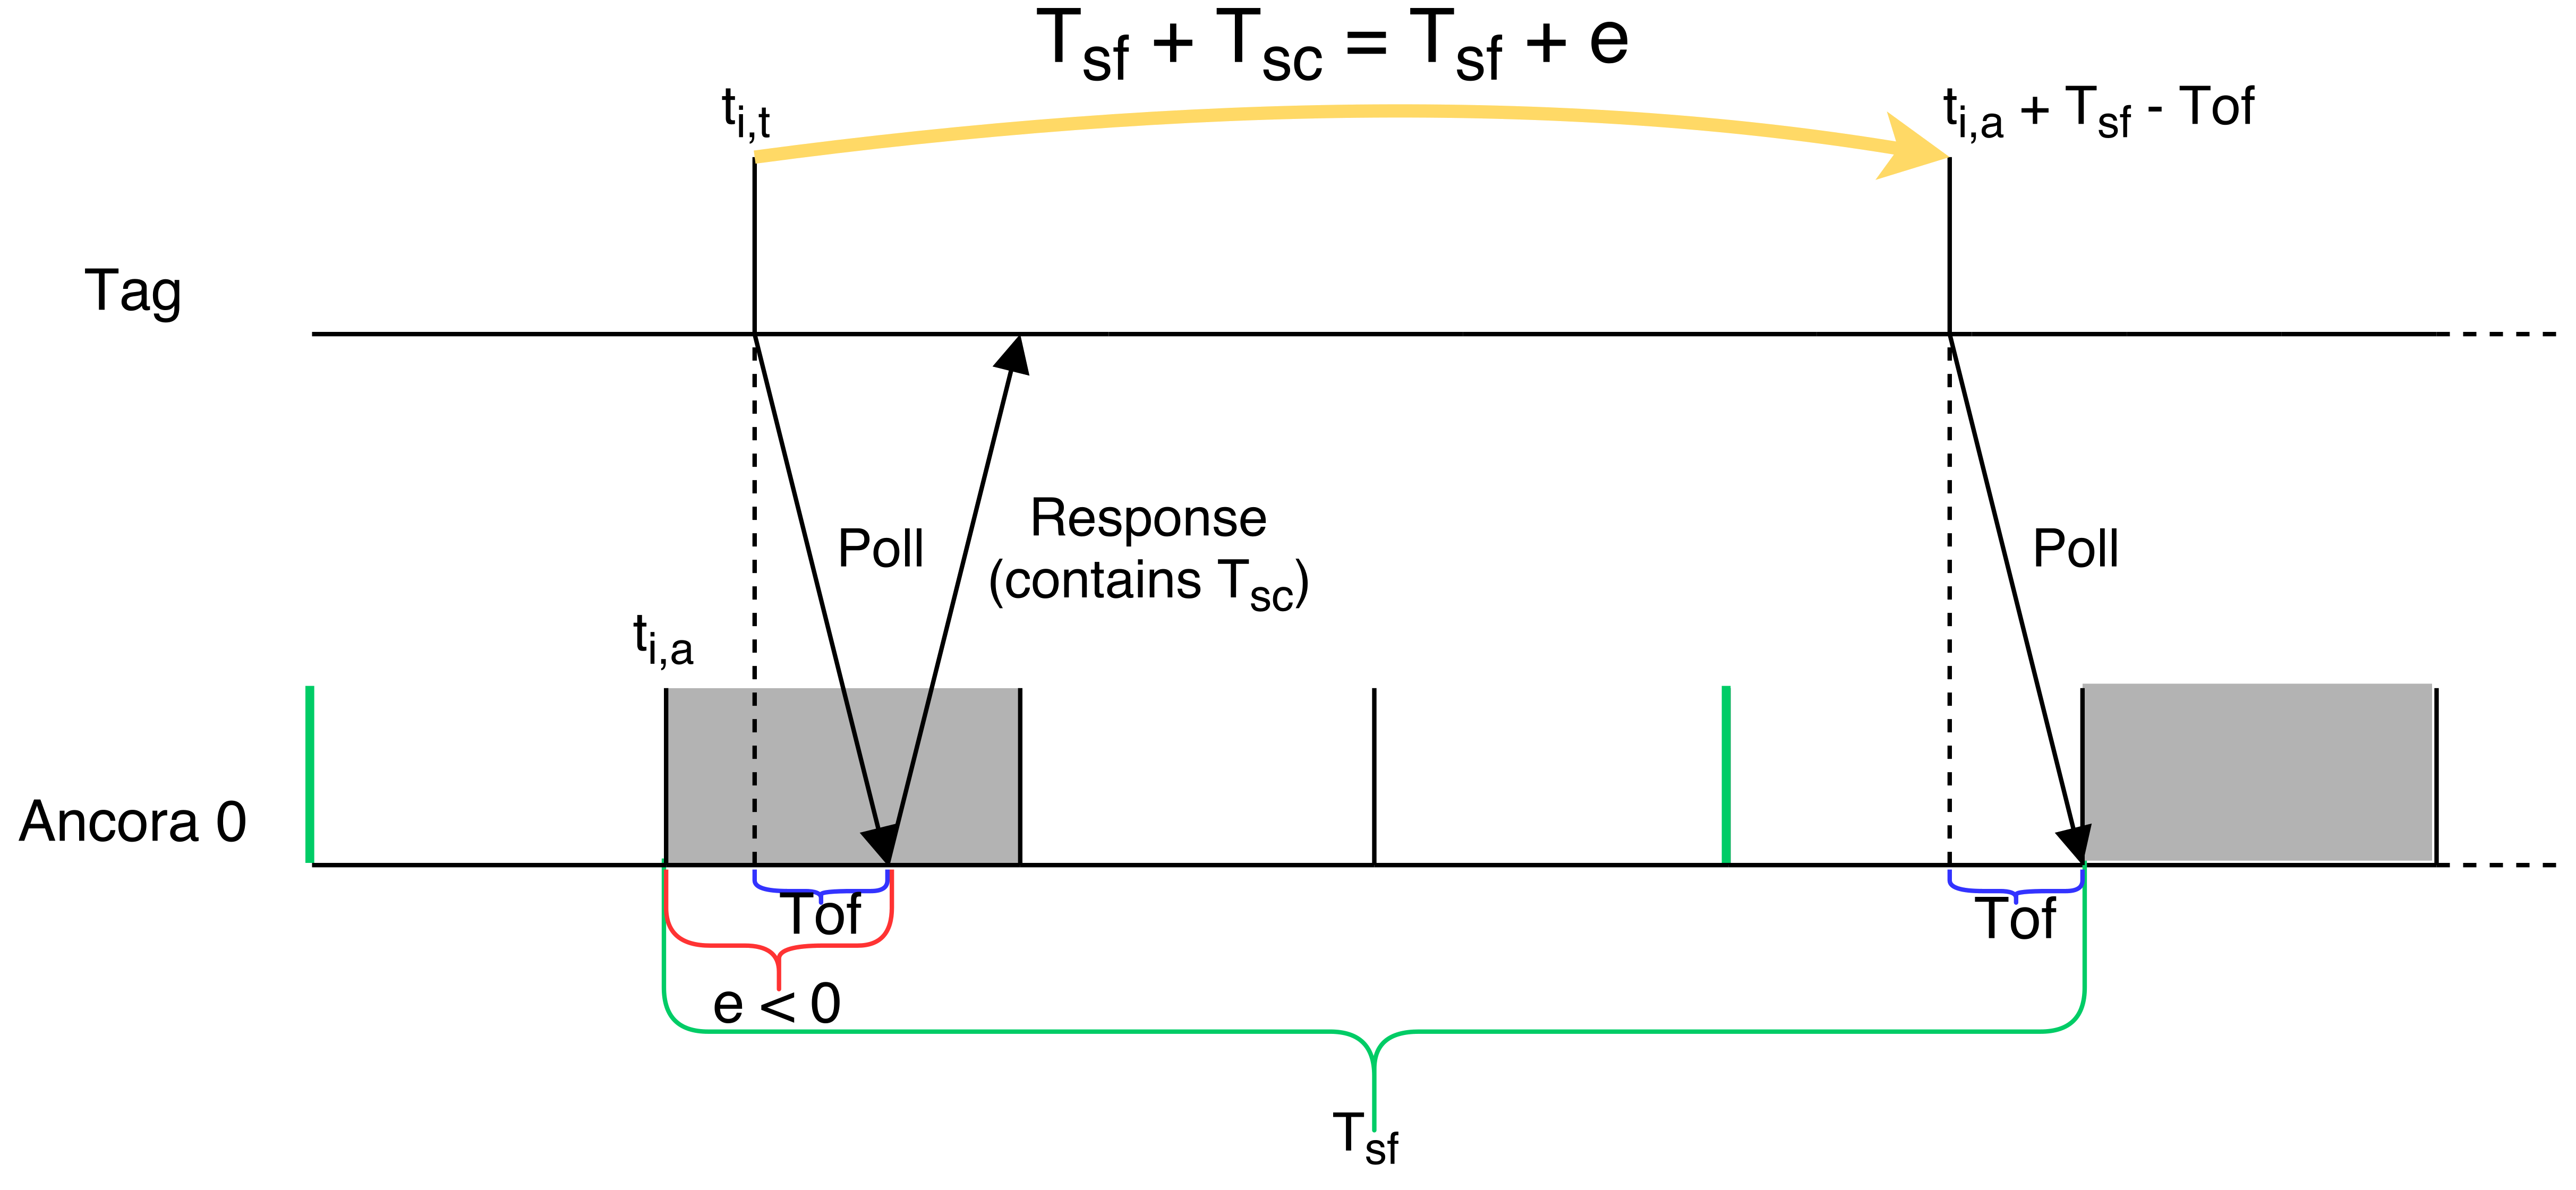
\includegraphics[width=\linewidth]{sleep_correction_less_half_superframe.png}
  \end{center}
\end{frame}

\begin{frame}{Calcolo del tempo di attivazione $T_{sc} = e + T_{sf}$}
  Nel seguente esempio si considera il caso $-\frac{T_{sf}}{2}$ \le e < 0$.\\
  Il tempo di riattivazione del tag $t_{i+1}^{t}$ è:
  \[
  t_{i+1}^{t} = t_{i}^{t} + T_{sf} + T_{sc} = t_i^a - (\cancel{e} + Tof) + T_{sf} + (\cancel{e} + T_{sf}) = t_i^a - Tof + 2T_{sf} 
  \]
  \begin{center}
    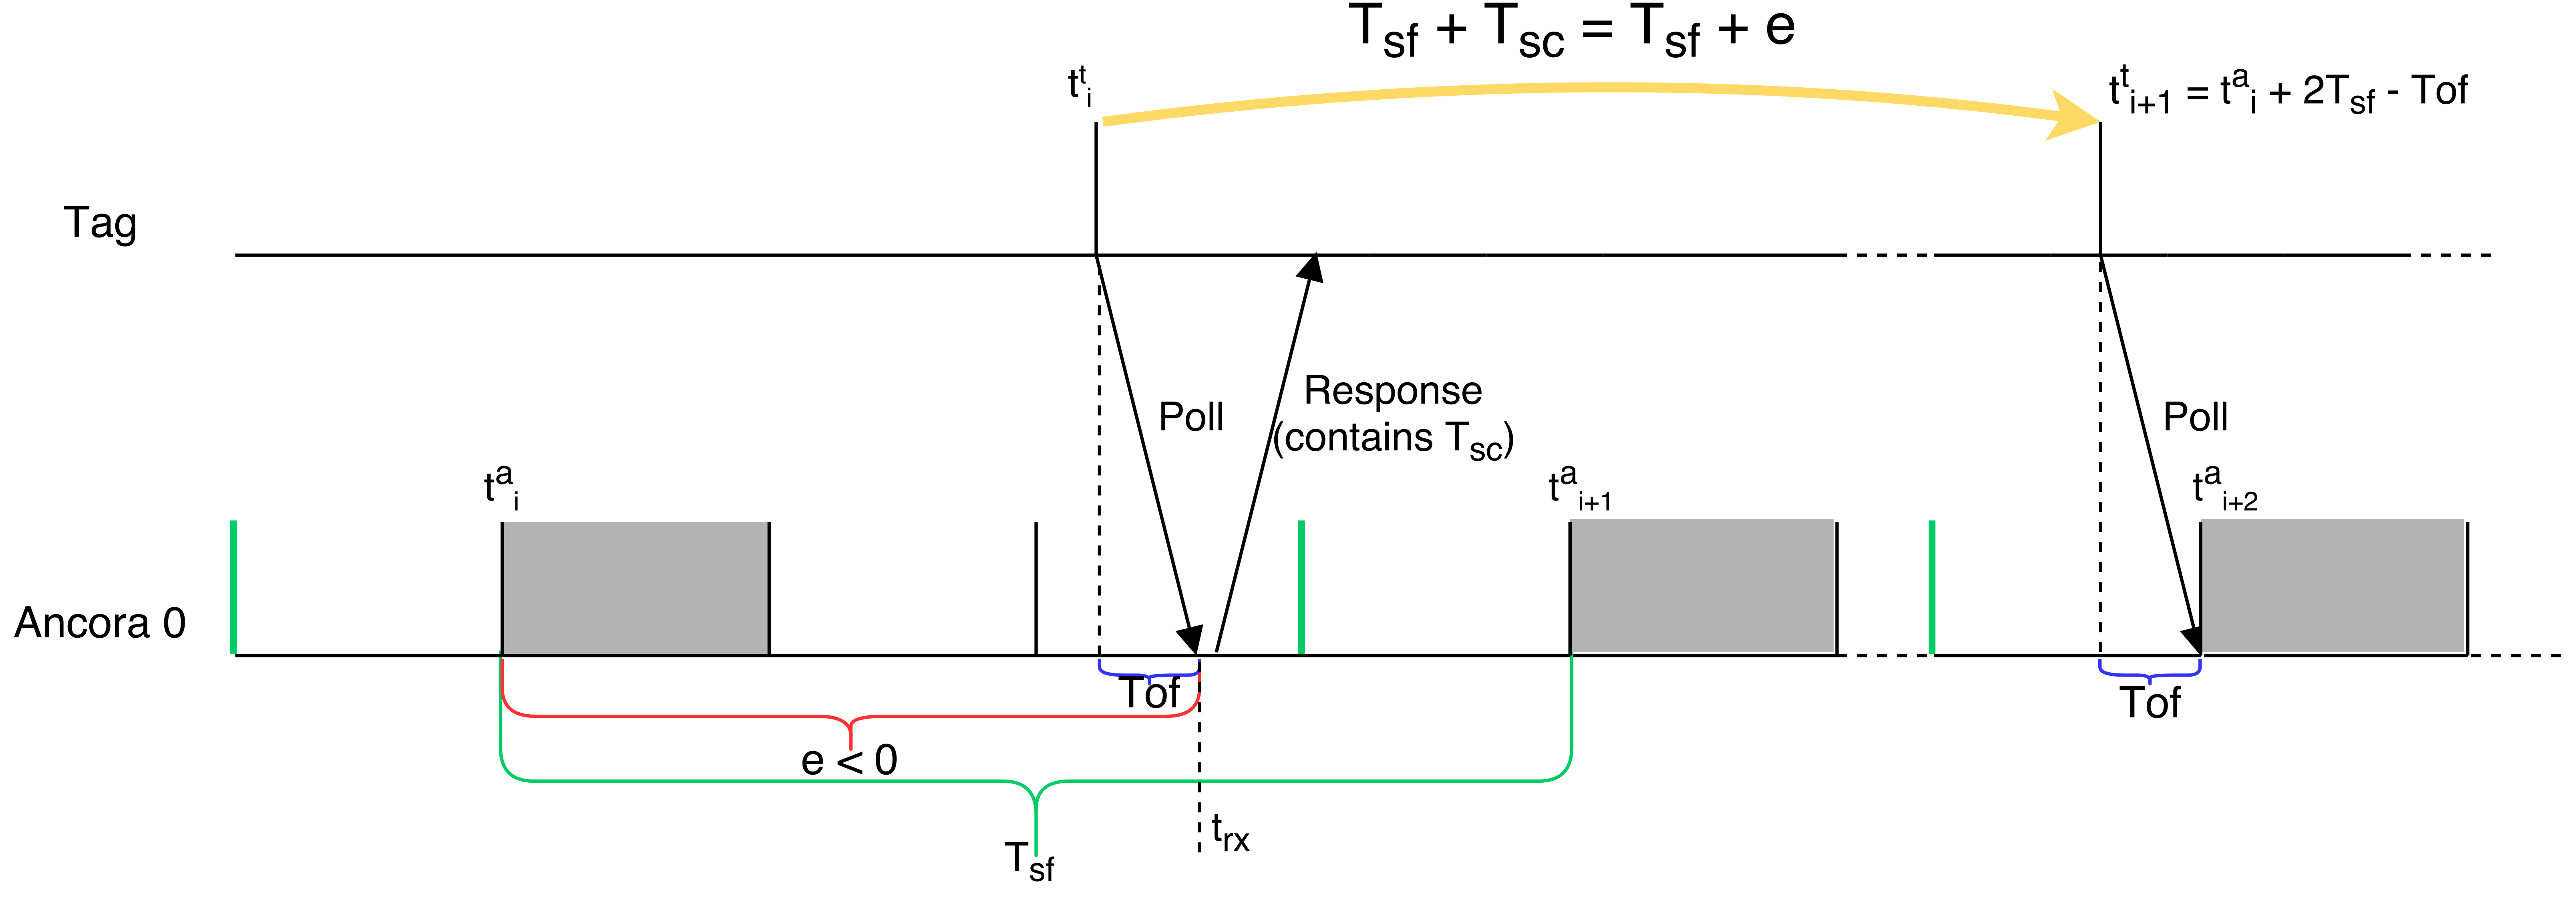
\includegraphics[width=\linewidth]{sleep_correction_greater_half_superframe.png}
  \end{center}
\end{frame}

\begin{frame}{Contributo di Pinna, Malagoli e Giannini}
  Dopo aver chiarito la struttura di frame e superframe è possibile comprendere
  il contributo degli studenti Pinna, Malagoli e Giannini.\\
  Al fine di aumentare la frequenza di ranging è stata ridotta la durata del superframe
  a quella di un solo frame.
  \begin{center}
    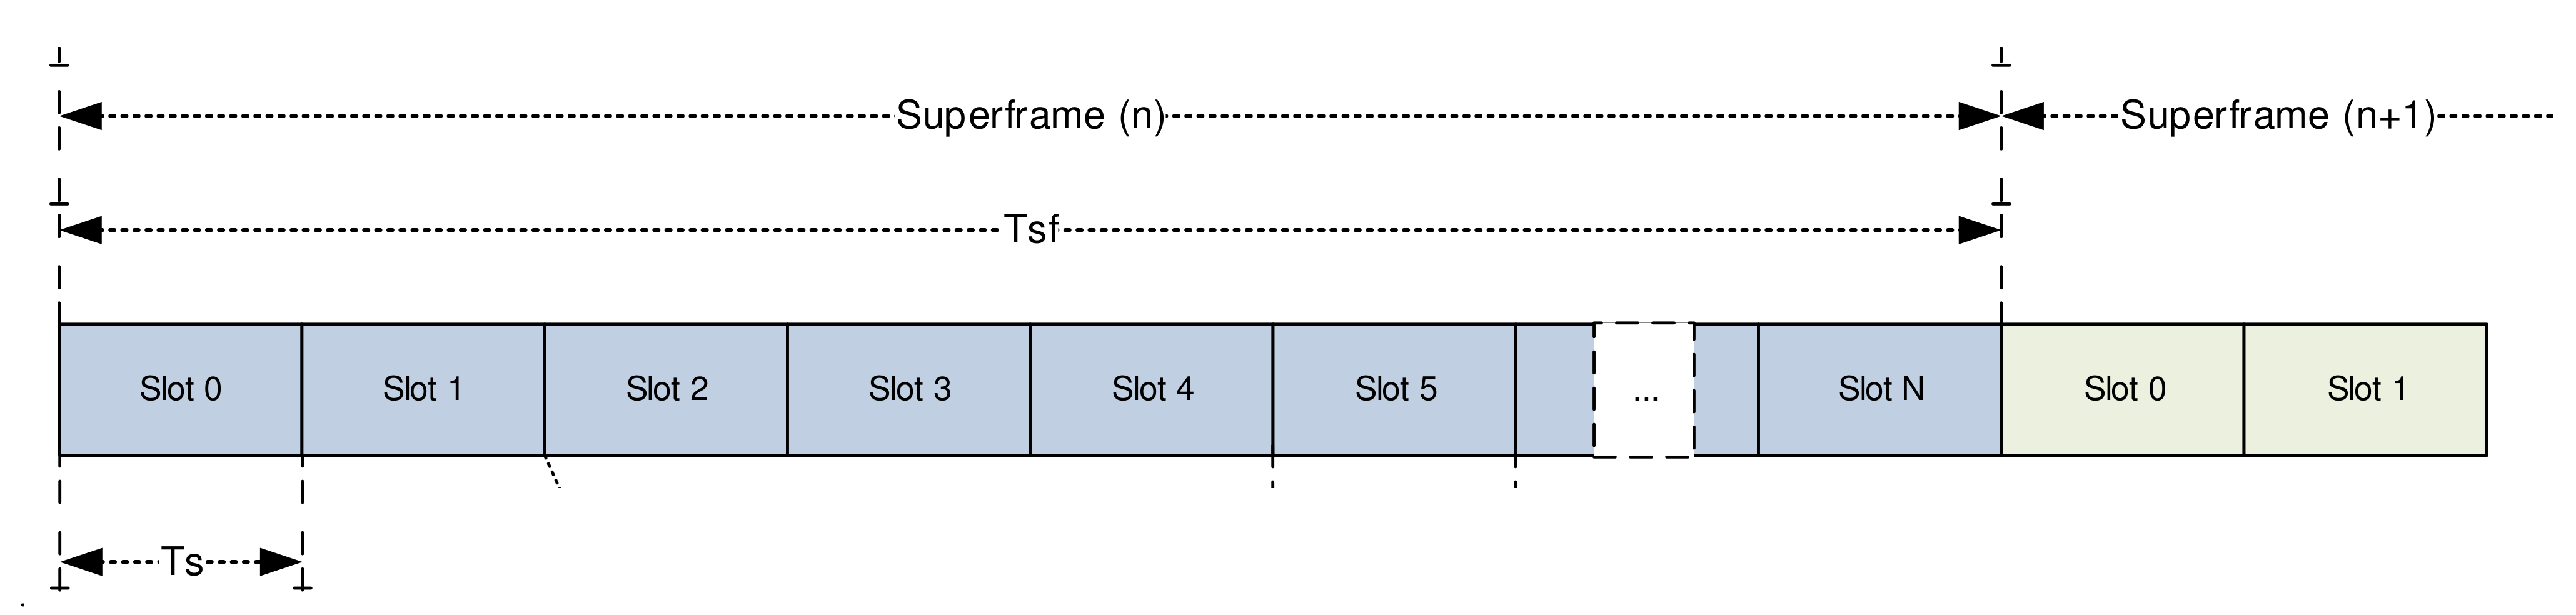
\includegraphics[width=\linewidth]{pmg_frames_removal.png}
  \end{center}
  In questa configurazione
  \begin{itemize}
  \item[-] il sistema è utilizzabile con un solo tag;
  \item[-] il tempo di superframe è $T_{sf} = T_s = \SI{10}{\milli\second}$;
  \item[-] la frequenza è $ f = \SI{100}{\hertz}$.
  \end{itemize}
\end{frame}

